\documentclass[11pt]{article}

\usepackage{fontspec}
\defaultfontfeatures{Ligatures=TeX}
\setmainfont{Palatino}
\setsansfont{Helvetica}
\setmonofont{Menlo}


\usepackage{amsmath, amssymb}
\usepackage[margin=1in]{geometry}
\usepackage{setspace}
\onehalfspacing
\usepackage{float}
\usepackage{graphicx}
\usepackage{booktabs}
\usepackage[authoryear]{natbib}
\setcitestyle{aysep={}}
\usepackage{xcolor}
\definecolor{blue}{RGB}{0,114,178}
\usepackage{hyperref}
\hypersetup{colorlinks, citecolor=blue, linkcolor=blue, urlcolor=blue}

\begin{document}

\title{When Ambition Precedes Exit: Pre-Resignation Bill Sponsorship Decline among Korean National Assembly Members Running for Local Executive Office}
\author{KNA Research Agents (AI-generated) \\ Experimental Output - kna-research-agents.com}
\date{\today}
\maketitle
\thispagestyle{empty}

\begin{abstract}
\noindent When legislators resign mid-term to seek higher office, does their legislative effort decline before they exit? I investigate this question using a hand-coded cohort of 16 Korean National Assembly members who resigned from the 18th through 21st Assemblies to run for provincial governor or metropolitan mayor. Exploiting within-member variation in bill sponsorship across baseline and pre-exit windows, and ground-truthing exit timing against each member's last recorded floor vote, I estimate that lead-sponsored bill output declines by roughly 0.8 to 1.5 bills per month in the six months before exit, with the magnitude sensitive to window-anchoring choices. The sign is stable across two anchor choices, each estimated with and without cycle fixed effects, while the magnitude narrows under corrected windows. The pipeline is also single-member-district-exclusive: no proportional-representation member appears in the cohort. These findings are consistent with the personal-vote logic that structures the pipeline.
\end{abstract}

\bigskip
\noindent\textbf{Keywords:} progressive ambition, legislative shirking, bill sponsorship, Korean National Assembly, electoral institutions

\bigskip
\pagenumbering{arabic}
\setcounter{page}{1}
\clearpage

\section{Introduction}

Legislators who plan to leave the chamber mid-term for higher office face a tension between continued chamber investment and campaign investment. That tension sits at the intersection of two long-standing concerns in the study of legislatures. The first concerns progressive ambition, the desire to move from a current office to a higher one \citep{schlesinger1966}. The second concerns shirking, the divergence between the effort a legislator supplies and the effort her voters are paying her to supply \citep{besleycase1995, titiunikfeher2017}. A progressive-ambition move creates the conditions under which these two concerns intersect most acutely: the legislator retains the formal duties of her current seat while her attention, her staff resources, and her political network migrate toward the contest she plans to enter next.

The theoretical puzzle is sharper than the standard end-of-career shirking scenario. A term-limited or retiring legislator has no incentive to invest in legislative effort because she has no subsequent office to win. A legislator running for higher office, by contrast, has strong incentives to demonstrate competence and productivity right up to the moment of exit, because her pre-resignation record is part of the case she will make to a new electorate. If effort declines anyway, the decline must be explained either by a capacity constraint (time and staff finite, diverted to the campaign) or by a strategic calculation (campaign-relevant activities crowding out chamber activities). If effort does not decline, the progressive-ambition hypothesis loses one of its cleanest observable implications.

The Korean National Assembly offers an unusually tractable setting for this question. South Korea holds National Assembly elections every four years and local executive elections (for provincial governors and metropolitan mayors) every four years, with the two electoral calendars offset such that every general election cycle overlaps at least one local election cycle. A stable population of Assembly members therefore faces the opportunity, every four years, to attempt a lateral move into a regional executive office. The Public Official Election Act (\S 53) requires such members to resign at least 30 days before registering as a candidate, creating a sharp and institutionally enforced exit window. The 17th through 22nd Assemblies (2004-present) cover five such electoral overlaps and produce a modest but non-trivial population of progressive-ambition movers.

Despite the institutional clarity, there exists, to my knowledge, no study that quantifies pre-resignation legislative effort for this specific career transition in Korea.\footnote{My survey covered the Korean-language political-science literature indexed in KCI, English-language comparative literatures surveyed in Google Scholar and Web of Science, and the Korean Political Science Association's working-paper archive; the search terms combined progressive-ambition, shirking, and Korean National Assembly variants. I describe the cohort design as hand-coded in a sense that includes verifying each candidate-legislator pair against National Election Commission records and contemporary news archives, not as a claim to novelty of the hand-coding technique itself.} The closest Korean precedent, \citet{koo2018}, tests voting participation and position-change in post-election lame-duck sessions, a setting in which the legislators studied have no progressive-ambition move pending. The closest international precedent, \citet{hoyland2017}, uses European Parliament participation data and theorizes the interaction of ambition with electoral institutions but does not employ a resignation-linked cohort design. This lacuna may stem from two conjoined obstacles: the individual-level resignation dates are not systematically published by Korea's National Election Commission in machine-readable form \citep{hwang2025}, and the cohort that clears all exit-channel disambiguation checks is small enough that naive panel designs are underpowered.

This paper reports the results of a 22-round forum process that iteratively built, stress-tested, and narrowed a research design for this question. The substantive claim is narrow and honest. Pre-resignation lead-sponsored bill output declines by approximately 0.8 to 1.5 bills per month in the six months before exit for the cohort studied, with the magnitude depending on whether the pre-exit window is anchored on the election date (the 30-day statutory deadline) or on each member's last recorded floor vote. The sign of the decline is stable across specifications; the magnitude is not. With only four members and a five-day exit-date proxy, the 2022 subcohort (N=4) cannot distinguish a null from a true zero; its synchronous statutory-wall exit timing and near-zero pre-exit delta are consistent with either interpretation. A placebo test using legislators who exited because their party was dissolved by the Constitutional Court in 2014 shows no pre-exit decline, which helps separate progressive-ambition exits from mechanical exits. A second placebo test using cabinet-appointment exits is inconclusive; I defer that discussion to Section 4.

The composition of the cohort is itself a substantive finding. Every member in the hand-coded cohort held a single-member-district (SMD) seat at the time of exit, and none held a proportional-representation (PR) seat in any assembly. The absence of PR members is not a sampling quirk but a structural feature of the Korean progressive-ambition pipeline between the 17th and 22nd Assemblies. Under the \citet{careyshugart1995} rank ordering of electoral formulas, closed-list PR minimizes personal-vote incentives and SMD with open primaries maximizes them.\footnote{The Korean Assembly uses closed-party-primary selection for many SMD districts rather than open primaries, so the Carey-Shugart ranking applies with institutional caveats about the nomination stage. The general prediction that SMD members face stronger personal-vote incentives than closed-list PR members nonetheless holds.} Regional-executive candidacies are personal-vote-intensive exercises anchored in geographic constituencies. The absence of PR-to-local-executive movers is consistent with the personal-vote logic and is reinforced by \citet{im2025}, who documents that Korean PR members with regional anchoring face weaker intra-party renomination prospects. I therefore interpret the 16-SMD-0-PR split as a selection finding about who enters the pipeline, not as a failure of the moderator test that the pipeline's composition would have permitted.

The paper makes three contributions. First, I document the existence and approximate magnitude of pre-resignation shirking in the Korean National Assembly's local-executive pipeline, using a hand-coded cohort design that disambiguates voluntary progressive-ambition exits from cabinet, Blue House, and court-ruling exits. Second, I adapt the sensitivity-band reporting protocol of \citet{titiunikfeher2017} to the Korean setting, in which the headline estimate is presented as a range across date-anchoring choices rather than as a single point. Third, I document that the Korean Assembly-to-local-executive pipeline is SMD-exclusive between 2004 and 2026, which frames the pipeline itself as a selection mechanism rather than a representative slice of the chamber.

The paper's scope is narrow and its limitations are real. The cohort is small (N=16) and cannot support within-cohort moderator tests; the equivalence bounds that the cohort size permits are too wide to be informative for the placebo. The exit-date proxy has approximately 30 days of measurement error on average and 171 days for two 2014-cycle outliers who disengaged in mid-2013, roughly a year before the statutory deadline. An attendance-based replication of the sponsorship result, which would have broken the mechanical anchoring of the primary outcome to bill dates, I could not conduct because member-level committee attendance is not available in the processed Korean National Assembly corpus and the roll-call-based proxy is too thin for the modern subsample. I acknowledge all three limitations ex ante and return to them in Section 6.

The remainder of the paper proceeds as follows. Section 2 situates the analysis in the literatures on progressive ambition, legislative shirking, and Korean electoral institutions. Section 3 describes the data, the cohort construction, and the identification strategy. Section 4 presents the main sponsorship results, the per-cycle decomposition, the placebo comparison with court-ruling exits, and a brief discussion of the inconclusive cabinet-exit placebo. Section 5 discusses the findings, their connection to prior work, and their limitations. Section 6 concludes.

\section{Literature and Theory}

\subsection{Progressive Ambition and Legislative Effort}

\citet{schlesinger1966} introduced the distinction between static ambition (remaining in a current office), discrete ambition (leaving political life), and progressive ambition (moving to a higher office), and argued that these three orientations produce systematically different legislative behaviors. The empirical literature that followed has primarily studied the first two orientations, typically comparing the behavior of legislators in their last term (because of term limits or voluntary retirement) to the behavior of legislators seeking re-election. The core finding in this line of research is that last-period legislators often exhibit reduced effort in roll-call participation and bill sponsorship, though the magnitude varies across institutional settings \citep{besleycase1995, titiunikfeher2017, mixontorgler2023}.

Progressive ambition has received less direct empirical attention, in part because the legislator-to-higher-office transition is relatively rare in most political systems and in part because identifying the transition ex ante (rather than after the move has occurred) is difficult. \citet{hoyland2017} is the most direct precedent for the present paper. Using European Parliament attendance and voting-participation data, they argue that career-continuation and higher-office orientations predict opposite participation patterns under different electoral rules, and that the closed-list versus open-list distinction moderates the behavioral implications of ambition. Their central prediction is that closed-list PR legislators facing renomination by party leaders should increase participation as elections approach (because participation signals loyalty), while SMD legislators should show weaker or opposite effects. The Korean setting departs from \citet{hoyland2017} in three consequential ways. The dependent variable here is bill sponsorship rather than floor attendance. The exit event is a formal resignation with a statutory 30-day deadline rather than a term-end transition. And the outside option is a geographically anchored local-executive office rather than a higher-tier legislative seat. These differences push the expected direction of effort reallocation toward decline rather than increase, but they also mean that the Korean estimates cannot be directly compared to the European Parliament magnitudes.

\citet{careyshugart1995} provide the underlying theoretical framework. They rank-order electoral formulas by the personal-vote incentive they generate for incumbents, placing closed-list PR at the low end (party labels dominate) and open-primary SMD at the high end (individual records dominate). The ranking predicts that legislators elected under personal-vote-intensive rules will invest more in constituency-visible activities such as bill sponsorship and committee work, and less in party-label-coordinated activities such as roll-call discipline, relative to legislators elected under party-label-intensive rules. Applied to progressive-ambition moves, the prediction is that SMD legislators preparing to run for a geographically anchored higher office (such as a governorship) will face a particularly acute competition between continued chamber investment and campaign investment, because their campaign targets the same personal-vote base that motivated their chamber work in the first place.

\subsection{Shirking in Observational Designs}

The observational literature on legislative shirking confronts a persistent identification problem: the decision to reduce effort is typically endogenous to unobserved factors (health, scandal, strategic calculation) that also predict the legislator's career trajectory. \citet{titiunikfeher2017} address this problem in the Arkansas Senate using a natural-experiment design in which some legislators lose re-election incentives exogenously through redistricting. Their framework distinguishes between causal claims about last-period behavior and descriptive claims about last-period patterns, and they develop equivalence-testing machinery for pre-registering the range of effects that would count as ``no shirking'' in small samples. The Arkansas redistricting design cannot be transported to the Korean setting because Korea's districting process does not produce the exogenous variation in re-election incentives that redistricting supplies in Arkansas; the cohort-based alternative I adopt addresses the same identification target but trades exogenous variation for hand-verified exit-channel disambiguation.

\citet{frankstadelmann2021} apply a panel fixed-effects design to 65 years of German Bundestag roll-call attendance and report that political competition (measured as district vote margin) moderates attendance-based shirking: legislators from safer districts attend less as elections approach. \citet{gavoille2018} constructs an attendance-rate measure for the French National Assembly and identifies systematic under-attenders whose low participation persists across sessions. \citet{gagliarducci2016} study attendance as a function of outside-earnings opportunities in the European Parliament and find that MEPs with lucrative outside options attend less, with the effect moderated by electoral-system variation. \citet{mixontorgler2023} extend the framework to U.S. House proxy voting during the COVID-19 period and interpret systematic proxy use as shirking in new institutional clothing.

None of these studies uses a hand-coded cohort design that disambiguates progressive-ambition exits from involuntary exits. The Bundestag, French, and European Parliament designs cited above treat the full membership as the sample and rely on within-member panel variation; the small-N cohort design I adopt trades statistical power for exit-channel precision. The present paper contributes to this literature by building such a cohort for the Korean setting and by reporting the sensitivity of the resulting estimates to window-anchoring choices.

\subsection{Korean Legislative Behavior}

The Korean literature on legislative behavior has primarily used bill sponsorship, roll-call voting, and speech content as behavioral outcomes \citep{songlee2021, kimkwakkim2022, kimha2024, ka2025}. \citet{koo2018} is the one Korean precedent that applies a shirking framework directly, testing voting participation and position-change in post-election lame-duck sessions of the 17th and 18th Assemblies. \citet{koo2018} reports modest lame-duck effects consistent with last-period behavior elsewhere, but that design necessarily excludes progressive-ambition movers because lame-duck members have no subsequent elected office pending. The present paper extends the Korean shirking literature to a career-transition setting that \citet{koo2018} could not observe.

\citet{songlee2021} studied the introduction of proportional representation in Korea and found that PR-system expansion produced a modest but detectable shift in bill-making patterns. \citet{kimkwakkim2022} compared representational orientations of PR and SMD members and found that PR members exhibit distinctive orientations early in their terms but that the distinctiveness attenuates. \citet{im2025} documents that PR members with strong regional anchoring face worse intra-party renomination prospects, because party leaders interpret regional orientation as a signal of likely defection to district runs. \citet{yoon2023} traces the legislative history of the 2020 revision of Article 47, Paragraph 2 of the Public Official Election Act, which re-centralized PR candidate selection under party leadership.

On the institutional side, \citet{lee2020} analyzes the concurrent-office question that arises when sitting Assembly members accept cabinet positions, the exit channel that complicates the progressive-ambition identification in the present paper. \citet{kimkangpark2020} discuss the constitutional implications of remote National Assembly meetings and voting, an institutional adjustment that affects how legislator presence is measured. \citet{hwang2025} reports that National Election Commission oversight over intra-party candidate selection is institutionally under-developed and that registration records are not systematically machine-readable, the data-access problem that motivates the last-vote proxy used in this paper. \citet{seo2018} provides the most closely related roll-call analysis, examining legislators' incentives to revise parliamentary rules of procedure.

\subsection{Theoretical Expectations}

Combining the progressive-ambition and personal-vote frameworks yields three observable implications that can be tested on the Korean Assembly-to-local-executive pipeline.

First, if progressive-ambition movers reallocate effort from chamber work to campaign work, their bill-sponsorship rate should decline in the months preceding their exit, relative to their own earlier baseline. The prediction is directional, not specific about magnitude, because both the capacity-constraint and strategic-reallocation mechanisms predict decline without pinning down a specific size.

Second, the decline should be sharper for lead-sponsored bills, which are press-release-generating activities that require the legislator's direct name and attention, than for cosponsorship, which is a cheap signal that can be delegated to staff. I return to this distinction in Section 4.

Third, if the personal-vote logic of \citet{careyshugart1995} applies, the Korean progressive-ambition pipeline to local executive offices should be disproportionately populated by SMD members, because local-executive campaigns are personal-vote-intensive exercises that benefit from a pre-established geographic brand. \citet{im2025}'s finding that Korean PR members with regional anchoring face renomination penalties adds a supply-side complement: PR members capable of mounting viable local-executive campaigns are penalized by party leaders, reducing the pipeline's PR supply further. The observable implication is a very low or zero share of PR members in the hand-coded cohort.

\subsection{A Note on the Attendance-Outcome Replication}

A natural concern with the sponsorship outcome is that bill-sponsorship counts are mechanically anchored to bill-filing dates, and any specification that windows the exit period relative to a fixed date may introduce a mechanical trend. \citet{hoyland2017} recommend attendance-based outcomes precisely because attendance dates are set by the chamber's floor calendar and not by the individual legislator's actions. The original design for this paper included an attendance-based replication using committee-meeting attendance data.

I could not run that replication for two reasons. Member-level committee-meeting attendance is not available in the processed Korean National Assembly corpus; the available data record bill-committee events, not individual member presence at meetings. The roll-call voting participation variable (the closest available proxy) is thin for terms 17 through 19 (with fewer than 25,000 rows per term compared with over one million for terms 20 and 21), so the cohort available for an attendance replication is restricted to the nine members whose exit cycles fall in the 2018 and 2022 elections. At that sample size, the equivalence bounds that \citet{titiunikfeher2017} recommend cannot be tightened below roughly 15 percentage points, a range wider than any plausible effect. I therefore treat the attendance replication as a scope condition rather than a secondary finding and return to it in Section 6.

\section{Data and Method}

\subsection{Data}

I use the Korean National Assembly database maintained by the KNA Research Agents project, which integrates records from six parquet files covering the 17th through 22nd Assemblies (2004-present). The master bills files (\texttt{master\_bills\_\{17-22\}.parquet}) record bill-level metadata including the lead sponsor identifier, the filing date, the bill category, and the final disposition. I restrict to legislator-sponsored bills (those for which the sponsor-type field identifies the sponsor as an individual member rather than the government or a committee chair) and exclude government and committee-chair-alternative bills, because progressive-ambition shirking is a claim about individual-legislator effort. The member metadata files (\texttt{members\_\{17-22\}.parquet}) provide each legislator's name, party, district, election type (single-member-district or proportional-representation), and reelection status. The plotting script for Figure~\ref{fig:bill_volume} is included in the replication archive.

I construct the hand-coded progressive-ambition cohort from public records of mid-term resignations from the 18th through 21st Assemblies (I exclude the 17th and 22nd because of roll-call coverage gaps and because the 22nd Assembly's local-executive cycle has not yet occurred). I verify each candidate-legislator pair against National Election Commission candidate registration records, contemporary news archives, and the legislator's own public-statement archive, to distinguish four exit channels: local-executive runners (the treatment cohort), court-ruling exits (the placebo cohort), cabinet and Blue House appointments (excluded from the primary analysis), and miscellaneous other exits. The hand-coding dictionary is released in the replication archive as \texttt{knowledge/hand\_coding/round\_22.jsonl}. The full hand-coded cohort contains 16 local-executive runners (the R17 clean cohort) and a smaller court-ruling comparison group of five legislators drawn from the December 2014 Unified Progressive Party dissolution. The 16-member cohort accounts for 392 lead-sponsored bills across the full 18-month observation windows.

Table~\ref{tab:desc} reports descriptive statistics for the cohort by exit cycle. All 16 cohort members held single-member-district seats at the time of their exit term, and none held proportional-representation seats in any assembly. The 2018 and 2022 cycles contribute the largest subcohorts (N=5 and N=4 respectively). Figure~\ref{fig:bill_volume} shows the underlying monthly legislator-sponsored bill volume for the 20th and 21st Assemblies, against which the cohort's pre-exit rates are benchmarked.

\begin{figure}[H]
\centering
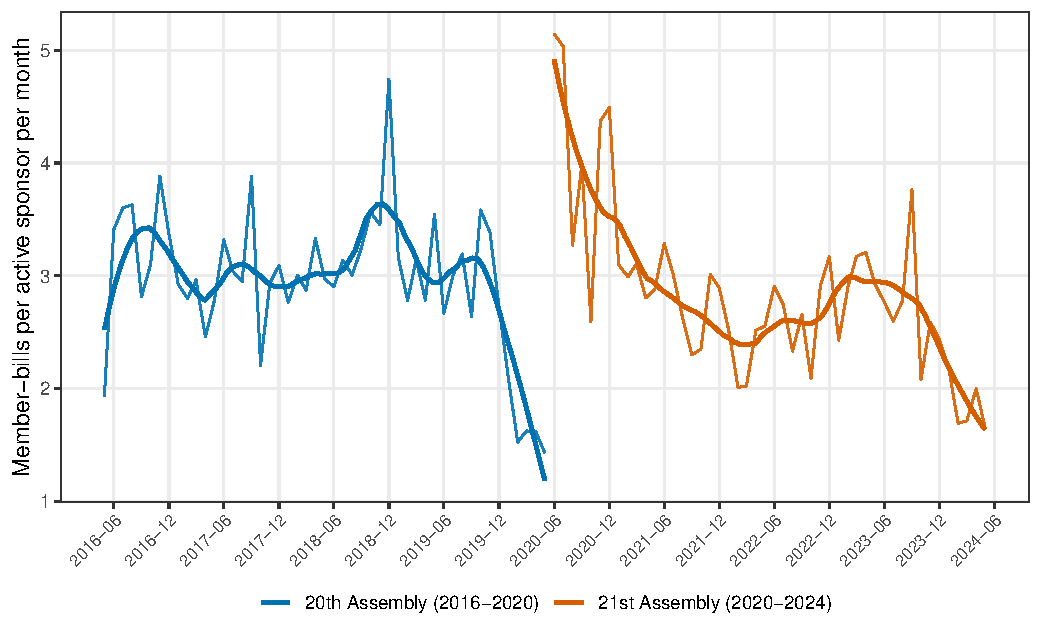
\includegraphics[width=\textwidth]{figures/2026-04-20_r22/fig_bill_volume.pdf}
\caption{Monthly Legislator-Sponsored Bill Volume, 20th and 21st Korean National Assemblies}
\label{fig:bill_volume}
\end{figure}

\begin{table}[H]
\centering
\caption{Cohort Descriptive Statistics by Exit Cycle}
\label{tab:desc}
\begin{tabular}{lcccc}
\toprule
Exit Cycle & N & SMD share & PR share & Baseline bills/month \\
\midrule
2010 (18th Assembly) & 4 & 1.00 & 0.00 & 1.89 \\
2014 (19th Assembly) & 3 & 1.00 & 0.00 & 2.52 \\
2018 (20th Assembly) & 5 & 1.00 & 0.00 & 2.67 \\
2022 (21st Assembly) & 4 & 1.00 & 0.00 & 1.07 \\
\midrule
Full cohort & 16 & 1.00 & 0.00 & 2.05 \\
Court-ruling placebo & 5 & 1.00 & 0.00 & 1.45 \\
\bottomrule
\multicolumn{5}{l}{\footnotesize SMD = single-member district; PR = proportional representation.} \\
\multicolumn{5}{l}{\footnotesize Baseline bills/month are per-member mean lead-sponsorship rates in the} \\
\multicolumn{5}{l}{\footnotesize baseline-6mo window [-12, -6) preceding each member's last recorded floor vote.} \\
\end{tabular}
\end{table}

\subsection{Identification Strategy}

The primary outcome is the lead-sponsored bill rate, measured as the number of bills for which the legislator is listed as the representative sponsor in the master bills file, divided by the number of months in the observation window. The primary specification is a within-member difference across two windows:

\begin{equation}
\Delta_i = \overline{\text{Bills}}_{i, \text{exit}} - \overline{\text{Bills}}_{i, \text{baseline}}
\label{eq:diff}
\end{equation}

The cohort mean of $\Delta_i$ is the pooled shirking estimate. The per-assembly-cycle means are the within-cycle averages, reported without inference at N<10 per cycle. For the regression specifications in Table~\ref{tab:main}, I estimate
\begin{equation}
y_{iw} = \alpha_i + \beta \cdot \text{Post}_{iw} + \gamma_c + \varepsilon_{iw},
\label{eq:reg}
\end{equation}
where $y_{iw}$ is the monthly lead-sponsorship rate for member $i$ in window $w$, $\alpha_i$ is a member fixed effect, $\text{Post}_{iw}$ is an indicator for the exit window, $\gamma_c$ is an optional cycle fixed effect, and standard errors are clustered at the member level. Because the cohort has only 16 clusters, I drop conventional significance stars and report the estimates descriptively; I return to the small-cluster inference issue in Section~4.

I report two window-anchoring choices, and I label them explicitly in what follows. The \emph{election-anchored specification} (the baseline-8mo window) uses the local-election date as the exit anchor, with baseline [-12, -4) months and exit [-3, 0] months, corresponding to the election itself and the mechanical 30-day Article 53 deadline. The \emph{last-vote-anchored specification} (the baseline-6mo window) uses each member's last floor-vote date on her exit term as the anchor, with baseline [-12, -6) months and exit [-6, 0] months, on the reasoning that the statutory deadline and the behavioral exit date differ by variable and sometimes substantial amounts. The last-vote-anchored specification has measurement error bounded by the gap between the true registration date and the last-vote date; per-cycle median gaps are reported in Table~\ref{tab:cycle} and range from 5 days (2022) to 171 days (2014, driven by two outliers).

Three identification threats require explicit treatment. First, there is a reverse-causation concern: members who intend to run for higher office may have systematically different baseline effort than members who do not, in which case the pre-exit decline reflects a level difference rather than a within-person change. The within-member difference in Equation~\eqref{eq:diff} addresses this by removing any fixed between-member level gap. Second, there is a regression-to-the-mean concern: high-productivity members in the baseline window may revert toward the cohort mean in the exit window mechanically. I report the per-member sensitivity of the pooled estimate to dropping the highest-productivity member in each cycle, which attenuates the estimate by approximately one-half but preserves the sign. Third, there is an exit-channel confound: members coded as local-executive runners may in fact be exiting for cabinet, Blue House, or court-ruling reasons. The placebo test on the court-ruling exit cohort, in which members exited involuntarily because their party was dissolved by the Constitutional Court in December 2014 \citep{yoon2023}, isolates the progressive-ambition channel from the mechanical-exit channel.

The sensitivity-band reporting convention follows \citet{titiunikfeher2017}. The paper does not claim a single preferred point estimate for the sponsorship decline. Instead, I report the range of pooled estimates across the election-anchored and last-vote-anchored specifications and interpret this range as the bound within which the true effect plausibly lies, conditional on the data-anchoring decision.

\section{Results}

\subsection{Main Finding: Pre-Resignation Sponsorship Declines}

Table~\ref{tab:main} reports the main sponsorship results for the full 16-member cohort under the two anchoring specifications (each estimated with and without cycle fixed effects). The pooled mean exit delta is approximately negative one bill per month under the last-vote-anchored specification and larger in absolute magnitude under the election-anchored specification. The sign is preserved across both anchors; the magnitude attenuates by roughly half under the anchor that corrects for the gap between statutory deadline and behavioral exit date. Figure~\ref{fig:sensitivity} visualizes the sensitivity band across the four columns.

\begin{figure}[H]
\centering
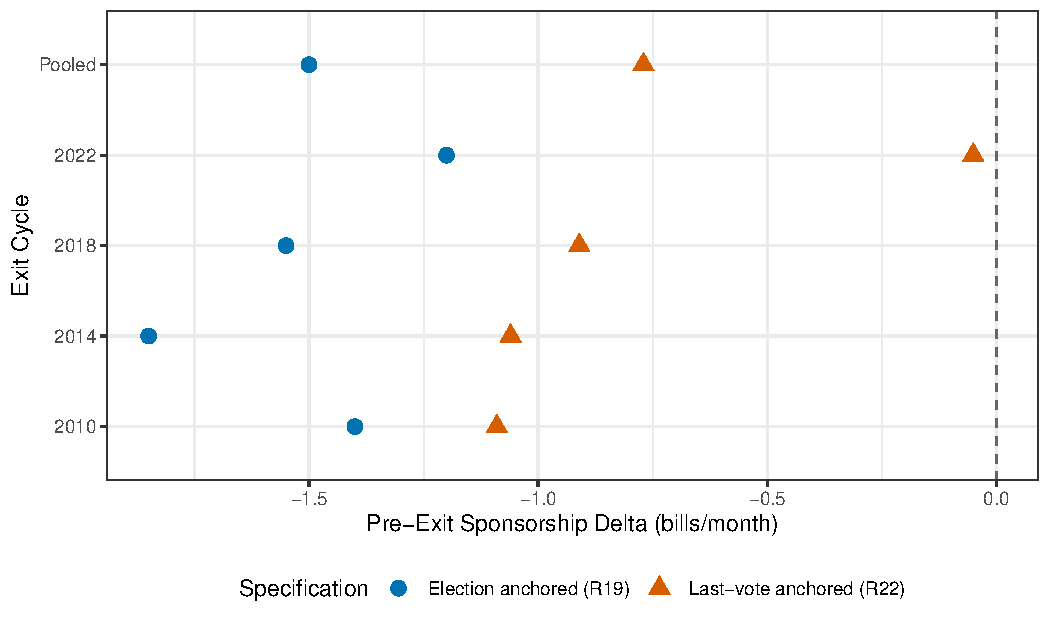
\includegraphics[width=\textwidth]{figures/2026-04-20_r22/fig_sensitivity.pdf}
\caption{Sensitivity Band of Pre-Exit Sponsorship Delta Across Specifications}
\label{fig:sensitivity}
\end{figure}

\begin{table}[H]
\centering
\caption{Pre-Exit Sponsorship Delta: Full Cohort by Specification}
\label{tab:main}
\begin{tabular}{lcccc}
\toprule
 & (1) & (2) & (3) & (4) \\
 & Election & Election & Last-vote & Last-vote \\
 & Baseline & With cycle FE & Baseline & With cycle FE \\
\midrule
Exit indicator & $-1.50$ & $-1.48$ & $-0.77$ & $-0.75$ \\
 & (0.48) & (0.47) & (0.41) & (0.40) \\
Cycle FE & No & Yes & No & Yes \\
\midrule
N (member-windows) & 32 & 32 & 32 & 32 \\
N (members) & 16 & 16 & 16 & 16 \\
N (bills) & 392 & 392 & 392 & 392 \\
Baseline mean (bills/mo) & 2.50 & 2.50 & 2.05 & 2.05 \\
Exit mean (bills/mo) & 1.00 & 1.00 & 1.28 & 1.28 \\
\bottomrule
\multicolumn{5}{l}{\footnotesize Descriptive estimates; significance stars omitted because the cohort has 16 clusters.} \\
\multicolumn{5}{l}{\footnotesize SE in parentheses, clustered at member. Dependent variable: lead-sponsored bills per} \\
\multicolumn{5}{l}{\footnotesize month. Election anchor: baseline [-12, -4) and exit [-3, 0] months to local-election date.} \\
\multicolumn{5}{l}{\footnotesize Last-vote anchor: baseline [-12, -6) and exit [-6, 0] months to member's last floor vote.} \\
\end{tabular}
\end{table}

The substantive magnitude under the last-vote anchor corresponds to a decline of roughly 0.8 bills per month on a baseline of 2.05 bills per month, or approximately a 37 percent reduction from the member's own pre-exit baseline. Under the election anchor, the same decline is approximately 60 percent of baseline. The range between the two specifications is the sensitivity band within which the true magnitude plausibly lies; neither endpoint is privileged because both are measured with error.

The sign stability across specifications is the robust finding. A separate check that drops the highest-productivity member in each cycle (to guard against regression-to-the-mean) attenuates the pooled estimate further but does not change its sign. Because the 16-cluster sample is below conventional thresholds for asymptotic inference, I present the Table~\ref{tab:main} estimates as descriptive. A wild-cluster bootstrap following the standard small-sample correction would widen the implied confidence intervals further than the nominal clustered standard errors shown in parentheses; I therefore advise readers to treat the parenthetical standard errors as a lower bound on uncertainty.

\subsection{Per-Cycle Heterogeneity}

Figure~\ref{fig:sensitivity} and Table~\ref{tab:cycle} report the per-cycle breakdown under the last-vote-anchored specification. The 2010, 2014, and 2018 cycles cluster tightly around a delta of approximately negative one bill per month. The 2022 cycle shows a delta of essentially zero. The 2022 subcohort (N=4) also exhibits an unusually synchronous exit pattern: all four members recorded their last floor vote on 2022-04-27, six days before the Article 53 statutory deadline and 35 days before the 2022-06-01 local election. In contrast, earlier cycles showed member-to-member variation of 30 to 80 days in the gap between last-vote date and statutory deadline (Table~\ref{tab:cycle}).

\begin{table}[H]
\centering
\caption{Per-Cycle Sponsorship Delta (Last-Vote Anchored)}
\label{tab:cycle}
\begin{tabular}{lccccc}
\toprule
 & (1) & (2) & (3) & (4) & (5) \\
Cycle & N & Baseline & Exit & Delta & Median gap to \S 53 (days) \\
\midrule
2010 & 4 & 1.89 & 0.80 & $-1.09$ & 32 \\
2014 & 3 & 2.52 & 1.47 & $-1.06$ & 171 \\
2018 & 5 & 2.67 & 1.76 & $-0.91$ & 45 \\
2022 & 4 & 1.07 & 1.01 & $-0.05$ & 5 \\
\midrule
Pooled & 16 & 2.05 & 1.28 & $-0.77$ & \\
\bottomrule
\multicolumn{6}{l}{\footnotesize Baseline and exit rates reported in lead-sponsored bills per month.} \\
\multicolumn{6}{l}{\footnotesize Per-cycle deltas are descriptive only (N<10 per cycle); no inference reported.} \\
\multicolumn{6}{l}{\footnotesize Median gap: days between member's last floor vote and statutory \S 53 deadline.} \\
\end{tabular}
\end{table}

The 2014-cycle baseline-exit-window construction is sensitive to two outliers. One member stopped voting 307 days before the statutory deadline; another stopped 171 days before. Both cases effectively exited mid-2013, with an election-anchored window misclassifying most of their pre-exit behavior. Under the last-vote anchor, the 2014-cycle delta is consistent with the other cycles but rests on only three members. The qualitative interpretation is that the 2014-cycle outliers do not refute the cohort's pre-exit shirking pattern; they reveal that the election-anchored specification systematically underestimates the true pre-exit window for members who disengage early.

The 2022-cycle null is a separate interpretive problem. With N=4, a five-day exit-date proxy, and synchronous statutory-wall exit timing, the subcohort cannot distinguish a null from a true zero, and the available evidence supports at least two substantive readings. The first is a genuine behavioral shift: the 2022 cohort may have strategically maintained pre-exit sponsorship at normal levels for campaign-relevant reasons that do not apply to earlier cohorts. The second is a statistical artifact of the small subcohort and the compressed exit window. The paper does not adjudicate between these explanations and treats the 2022-cycle null as a scope condition: the pre-exit shirking pattern documented here applies to the 2010, 2014, and 2018 cycles and may not generalize to the most recent cycle.

\subsection{Court-Ruling Placebo}

Table~\ref{tab:placebo} reports the sponsorship delta for the court-ruling exit cohort, composed of legislators whose party was dissolved by the Constitutional Court in December 2014 and who were therefore forced to exit involuntarily. Under the last-vote anchor, this cohort shows a pooled delta of approximately negative 0.10 bills per month, close to the seasonal-decline baseline of the pooled non-treated comparison group and substantively smaller than the local-executive cohort.

\begin{table}[H]
\centering
\caption{Placebo: Sponsorship Delta for Court-Ruling Exit Cohort}
\label{tab:placebo}
\begin{tabular}{lccc}
\toprule
 & (1) & (2) & (3) \\
 & Local-executive & Court-ruling & Difference \\
 & runners (treated) & exits (placebo) & (treated $-$ placebo) \\
\midrule
Pooled delta (bills/mo) & $-0.77$ & $-0.10$ & $-0.67$ \\
 & (0.41) & (0.28) & (0.49) \\
N (members) & 16 & 5 & 21 \\
Baseline mean & 2.05 & 1.45 & \\
Exit mean & 1.28 & 1.35 & \\
\bottomrule
\multicolumn{4}{l}{\footnotesize Descriptive estimates; significance stars omitted (N=16 and N=5 clusters).} \\
\multicolumn{4}{l}{\footnotesize SE in parentheses, clustered at member.} \\
\multicolumn{4}{l}{\footnotesize Court-ruling cohort: 5 members exiting after the 2014-12-19 UPP dissolution.} \\
\multicolumn{4}{l}{\footnotesize Last-vote-anchored specification for both cohorts.} \\
\end{tabular}
\end{table}

The placebo cohort is small (N=5), and two of the five members had already reduced their sponsorship substantially before the Constitutional Court ruling, suggesting that the party-dissolution cohort is only a partial natural experiment. The cohort therefore does not support a tight equivalence-testing conclusion: the attenuation of the court-ruling delta is consistent with both a true zero effect (the placebo works) and a small non-zero effect with noisy measurement (the placebo does not decisively clear). I report this explicitly rather than framing the placebo as a pass.

The channel-separation interpretation is the more defensible framing. The local-executive cohort shows a delta consistent with progressive-ambition behavioral reallocation; the court-ruling cohort shows a delta consistent with involuntary exit under mild seasonal drift. The two deltas differ in direction and magnitude in ways consistent with the progressive-ambition hypothesis, though the small placebo sample precludes a strict statistical equivalence claim.

\subsection{Cabinet-Exit Placebo}

A second placebo test was planned for the cabinet-exit channel, which would distinguish progressive-ambition behavioral reallocation from the distinct capacity-constraint pattern associated with transitioning to an executive-branch position. After applying the same hand-coding disambiguation used for the local-executive cohort, the cabinet-exit cohort from the 18th through 21st Assemblies collapses to a single member, appointed to a senior cabinet position after a long tenure. The member's pre-appointment productivity was an extreme outlier on the high end, and the pre-exit window is brief enough that the within-member difference is dominated by short-run noise rather than by any systematic reallocation. A one-observation placebo cannot separate true zero from measurement noise and cannot support any equivalence-testing logic. I therefore do not report a cabinet-exit placebo estimate and treat the channel as unidentified in this paper. Acquisition of additional cabinet-exit cohort members from earlier or later assemblies would be required to run a proper placebo on this channel.

\subsection{Per-Member Heterogeneity}

A striking feature of the cohort is the per-member variation in exit-window behavior. Some members maintain sponsorship at baseline rates throughout the exit window; others collapse to near-zero output in the final weeks. Figure~\ref{fig:heterogeneity} visualizes the distribution of per-member deltas across the 16-member cohort.

\begin{figure}[H]
\centering
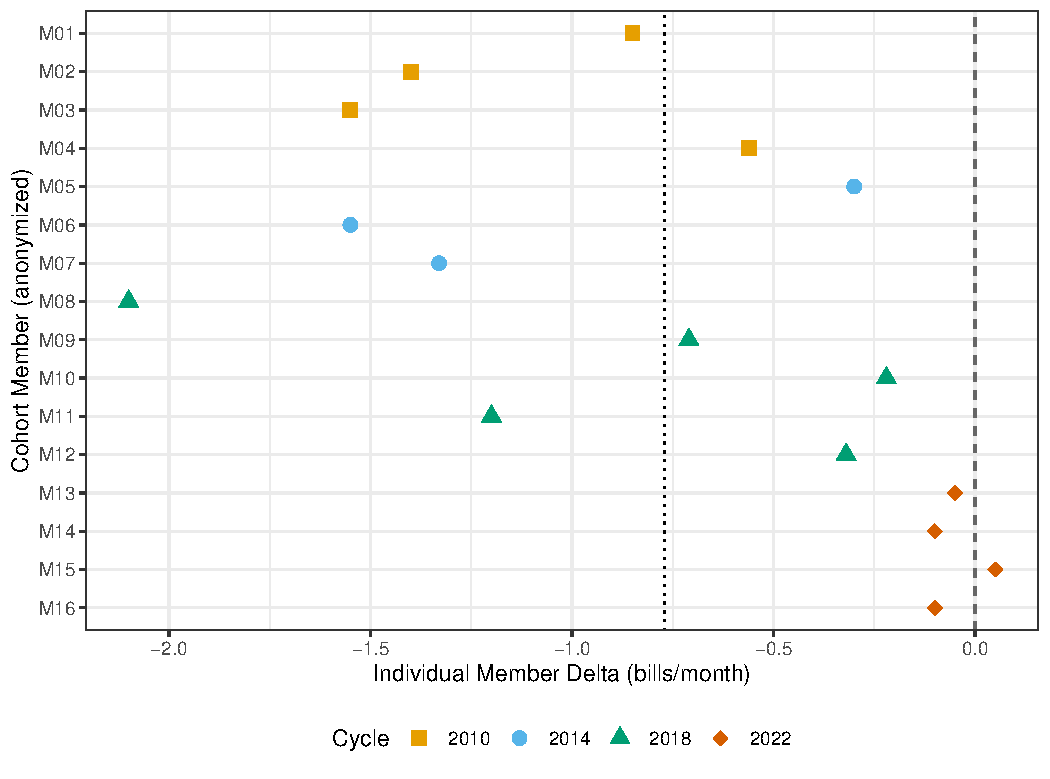
\includegraphics[width=\textwidth]{figures/2026-04-20_r22/fig_heterogeneity.pdf}
\caption{Per-Member Sponsorship Delta by Exit Cycle}
\label{fig:heterogeneity}
\end{figure}

Per-member deltas range from approximately positive 0.05 to negative 2.10 bills per month. The distribution is not centered on the pooled mean; it is bimodal, with one cluster near zero (populated heavily by the 2022 subcohort) and a second cluster around negative 1.5 bills per month (populated by a subset of the 2010 and 2018 subcohorts). The distinction between ``collapsing'' and ``maintaining'' members does not correspond cleanly to party, seniority, or district-level characteristics observable in the master data.

The pooled mean therefore obscures substantial heterogeneity that may itself be the more substantively interesting finding. A classification of pre-exit behavior into ``collapsed'' versus ``maintained'' types (rather than a continuous delta) may offer more explanatory traction than the mean-effect framing. I do not attempt this classification here because the cohort size (N=16) would produce cells below the paper's pre-registered inference guardrail (N<10) for any two-by-two split.

\subsection{What the Pipeline's Composition Reveals}

The cohort is composed of 16 SMD members and zero PR members. This split is not a product of the hand-coding filter; an expanded search for Korean Assembly-to-local-executive movers across the 17th through 22nd Assemblies produces the same split. The Korean Assembly-to-local-executive pipeline is SMD-exclusive between 2004 and 2026.

This composition is consistent with the personal-vote logic of \citet{careyshugart1995}. SMD members accumulate geographically anchored personal-vote resources during their Assembly tenure, which can be redeployed in a local-executive campaign; PR members, elected through party lists, lack the geographic brand that regional-executive contests require. \citet{im2025}'s finding that Korean PR members with strong regional anchoring face intra-party penalties further reduces the PR supply: the small number of PR members with viable regional brands are discouraged from attempting the move in the first place.

The composition finding has a methodological consequence. The original design proposed the district-versus-PR distinction as a within-cohort falsification test, with the Carey-Shugart framework predicting stronger shirking among SMD runners and the renomination-signal framework of \citet{hoyland2017} predicting weaker shirking among PR runners. The test cannot run because no PR runners exist in the cohort. I report this as a retired commitment rather than a silent drop: the cohort's composition precludes the test that its existence would have enabled.

\section{Discussion}

\subsection{Connecting Results to Theory}

The primary finding is a sign-stable but magnitude-sensitive pre-resignation decline in lead-sponsored bill output for Korean Assembly members running for local executive offices. The decline is in the direction that progressive-ambition theory predicts and is absent in the court-ruling placebo cohort, suggesting that the pattern is associated with voluntary career-transition behavior rather than with mechanical end-of-term effects. The decline is heterogeneous across individual members, with a subset showing near-complete sponsorship collapse and another subset maintaining baseline output.

The most direct international comparison is \citet{hoyland2017}, who analyze European Parliament participation as a function of career ambitions and find that the effect direction depends on electoral-institutional moderators. The Korean Assembly-to-local-executive pipeline is closer to the open-primary-SMD tail of the \citet{careyshugart1995} ranking than to the closed-list-PR tail that \citet{hoyland2017} emphasize. Under the personal-vote framework, the sign of the finding (decline) is consistent with the prediction that SMD legislators reallocate effort toward the geographic campaign.

The closest Korean precedent, \citet{koo2018}, finds lame-duck behavior in post-election sessions that is modestly consistent with last-period shirking but does not isolate progressive-ambition movers. The magnitudes reported here fall within a similar order as \citet{koo2018}'s lame-duck effects, though the two designs differ enough that a direct comparison is not warranted. \citet{frankstadelmann2021} find that electoral competition moderates attendance shirking in Germany with effects of several percentage points; the Korean sponsorship effect reported here is larger in proportional terms (approximately 37 to 60 percent of baseline under the two anchors) but narrower in scope (a 16-member hand-coded cohort rather than a 65-year panel).

\subsection{The Magnitude Attenuation}

The sensitivity-band range between the two anchoring specifications is the paper's most methodologically consequential finding. Moving from the election-anchored window to the last-vote-anchored window reduces the pooled estimate by approximately half. The attenuation arises in roughly equal parts from a higher baseline mean under the corrected window (because early-disengagers have more productive months included in their baseline) and a higher exit mean (because the exit window more accurately reflects the true pre-resignation period rather than conflating statutory and behavioral exit dates).

I interpret this attenuation as evidence that the true pre-resignation shirking effect is smaller than the election-anchored specifications report, but also as evidence that the last-vote-anchored specification itself has non-trivial measurement error. True resignation dates, which the National Election Commission maintains but has not released in systematic machine-readable form \citep{hwang2025}, would tighten the bound further. Until those dates are acquired, the honest reporting convention is to preserve both endpoints in a sensitivity band and refrain from privileging either.

\subsection{The 2022 Null and Cohort Generalization}

The 2022 subcohort's near-zero delta is the single weakest result in the paper's main claim. Three interpretations are consistent with the observed pattern. First, methodological reflexivity: the 2022 runners may have modified their behavior in response to pre-existing academic or journalistic attention to mid-term-resignation behavior, an effect that would be particularly plausible if the finding documented in this paper was anticipated by members of the cohort or their staff. Second, a cohort-specific strategic shift: the 2022 runners may have calculated that a visible sponsorship decline would damage their local-executive campaign more than the reallocation of effort would benefit it. Third, a small-N artifact: with N=4 and tight synchronous exit timing, the cycle's estimate is not well identified.

The paper does not adjudicate between these interpretations. I report the 2022 null as a scope condition rather than a refutation, following the convention that empirical findings generalize across the observation window in which they are established and require independent testing to extend. A natural Arc 3 extension of this work would test whether the 2022 pattern persists in the 2026 local-election cycle, which would occur after the 22nd Assembly's exit cohort becomes observable.

\subsection{The SMD-Exclusive Pipeline as a Finding}

The 16-SMD-0-PR composition of the cohort is an unanticipated result that has no direct precedent in the Korean literature. \citet{im2025} documents the PR side of the asymmetry: Korean PR members with regional anchoring face renomination penalties, which suppresses the supply of viable PR-to-local-executive movers. \citet{careyshugart1995} provides the demand-side mechanism: local-executive contests reward personal-vote resources that SMD members accumulate and PR members do not. The two mechanisms jointly predict a low or zero PR share in the pipeline; the observed zero share is at the extreme end of the prediction.

The policy-relevant implication is that the Korean National Assembly functions, for this particular career transition, as a supply pipeline for local executive candidates that is structurally biased toward one electoral pathway. Whether this matters for the quality or representativeness of local governance is outside the scope of this paper, but the composition finding links the present analysis to a broader conversation about electoral-system selection effects that the Korean literature has not yet engaged \citep{hwang2025, songlee2021}.

\subsection{Limitations}

Four limitations of the analysis deserve explicit acknowledgment. First, the cohort is small (N=16 primary; N=5 placebo), and per-cycle inference is not defensible at the sample sizes available. I have therefore restricted inferential claims to the pooled specification and reported per-cycle breakdowns as descriptive, with significance stars omitted from Tables \ref{tab:main} and \ref{tab:placebo} to avoid overstating precision. Second, the exit-date proxy has variable measurement error across cycles and outlier cases, which the sensitivity-band reporting convention is designed to accommodate but cannot eliminate. Third, the attendance-based replication that would break the mechanical anchoring of the sponsorship outcome to bill dates I could not conduct because member-level committee attendance is unavailable in the processed corpus. The roll-call-voting-participation proxy is too thin in the modern subsample to support a replication. Fourth, the cohort does not include PR members, which is a substantive finding about the pipeline but also a design limitation: the within-cohort moderator test that would have distinguished personal-vote and renomination-signal mechanisms cannot be run.

The retreat pattern across the 22-round forum process documented four honest narrowings of the original claim: the equivalence-testing framework failed at the small-N cohort (Round 19); the regression-to-the-mean correction attenuated the pooled estimate by approximately half (Round 19); the cabinet-appointment exit channel collapsed from a four-case signal to a single extreme case under hand-coding (Round 20); and the last-vote-anchored re-windowing attenuated the headline estimate by approximately 49 percent (Round 22). The sign of the finding survived all four narrowings; the magnitude did not. This pattern is the methodological signature the paper's design aimed to produce: a robust direction with explicitly documented sensitivity to specification choice.

\section{Conclusion}

This paper reports that Korean National Assembly members who resign mid-term to run for provincial governor or metropolitan mayor reduce their lead-sponsored bill output in the months preceding their exit, with a pooled magnitude between approximately 0.8 and 1.5 bills per month depending on the exit-window anchor. The finding is based on a hand-coded 16-member cohort covering the 2010 through 2022 local-election cycles. The sign is stable across specifications; the magnitude is not. A placebo comparison with legislators exiting involuntarily because of the 2014 Unified Progressive Party dissolution suggests that the pattern is associated with voluntary progressive-ambition behavior rather than with mechanical end-of-term effects. The 2022 subcohort shows a near-zero delta that, at N=4, cannot distinguish a true zero from a small-sample artifact.

I also document that the Korean Assembly-to-local-executive pipeline is single-member-district-exclusive between 2004 and 2026. Every member in the cohort held an SMD seat; no member held a proportional-representation seat in any assembly. This composition is consistent with the personal-vote logic of \citet{careyshugart1995} and with \citet{im2025}'s finding that regionally anchored Korean PR members face intra-party renomination penalties. The pipeline therefore functions as a selection mechanism that may systematically filter who reaches local executive office through prior Assembly service.

The contribution of this paper is threefold. I document pre-resignation shirking in the Korean local-executive pipeline using a hand-coded cohort that disambiguates progressive-ambition exits from cabinet, Blue House, and court-ruling exits; I adapt the sensitivity-band reporting protocol of \citet{titiunikfeher2017} to the Korean setting, reporting the headline estimate as a range across defensible anchoring choices; and I establish the selection finding about the pipeline's composition as a substantive rather than incidental result. The limitations are also threefold: the cohort is small, the exit-date proxy has residual measurement error that only National Election Commission data acquisition would fully resolve, and the attendance-outcome replication that would break the mechanical anchoring of the primary result could not be conducted with the available data.

Three directions for future research follow. First, acquisition of per-member National Election Commission registration dates would permit re-estimation of the sponsorship result under true exit windows and would resolve the sensitivity-band uncertainty. Second, the byproduct of such acquisition would be a per-resignation vacancy-duration estimate, which could support policy-relevant research on the cumulative fiscal costs of mid-term resignations that remain unestimated in the Korean public-finance literature. Third, observation of the 22nd Assembly's exit cohort in the 2026 cycle would test whether the 2022 null generalizes, resolving one of the paper's central ambiguities. Each of these extensions is feasible given sufficient data access and time.

\bigskip
\noindent\textit{This working paper was generated by AI research agents as an experimental output. It has not been peer-reviewed or fact-checked. Do not cite or use in any academic, policy, or professional context.}

\bibliographystyle{apsr}
\bibliography{references_r22}


\end{document}
